% =====================================================================
%  Rapport du projet POO : moteur masses-ressorts (Phelma 3A SEI)
%  Charte reprise du diaporama (assets/presentation) : memes couleurs,
%  memes polices, memes schemas draw.io (figures/schemas/*.pdf).
%
%  Compilation :  make        -> build/rapport.pdf
% =====================================================================
\documentclass[11pt,a4paper]{article}

\usepackage[utf8]{inputenc}
\usepackage[T1]{fontenc}
\usepackage[french]{babel}
\usepackage{tgheros}
\usepackage[scaled=0.86]{FiraMono}
\renewcommand{\familydefault}{\sfdefault}
\usepackage{amsmath,amssymb}
\usepackage{sansmath}\sansmath
% sansmath n'a pas de glyphe << vecteur >> (il sort un tilde) : vraie fleche
\renewcommand{\vec}[1]{\overset{\scriptscriptstyle\rightarrow}{#1}}

\usepackage[a4paper,margin=2cm,top=2.3cm,bottom=2.2cm,headheight=14pt]{geometry}
\usepackage{graphicx}
\usepackage{xcolor}
\usepackage{booktabs,array,tabularx}
\usepackage{caption}
\usepackage{enumitem}
\usepackage{fancyhdr}
\usepackage{titlesec}
\usepackage{listings}
\usepackage{tikz}
\usetikzlibrary{calc,positioning,arrows.meta,babel}
\usepackage{pgfplots}
\pgfplotsset{compat=1.18}
\usepackage{fontawesome5}
\usepackage[hidelinks]{hyperref}

% ------------------------------------------------------------- couleurs
\definecolor{phelmared}{HTML}{BD1D1D}
\definecolor{inpnavy}{HTML}{2A2E47}
\definecolor{timaorange}{HTML}{E76F51}
\definecolor{astblue}{HTML}{336CE6}
\definecolor{astframefill}{HTML}{F5F7FB}
\definecolor{memborder}{HTML}{336CE6}   \definecolor{memfill}{HTML}{E0F2FE}
\definecolor{ctrlred}{HTML}{DC2626}     \definecolor{ctrlfill}{HTML}{FEE2E2}
\definecolor{dummyorange}{HTML}{D79B00} \definecolor{dummyfill}{HTML}{FFE6CC}
\definecolor{datagreen}{HTML}{82B366}   \definecolor{datafill}{HTML}{D5E8D4}
\definecolor{sinkpurple}{HTML}{9673A6}  \definecolor{sinkfill}{HTML}{E1D5E7}
\definecolor{combislate}{HTML}{23445D}
\definecolor{floorgrey}{HTML}{AAACAD}
\definecolor{textgrey}{HTML}{5F6368}
\colorlet{astrulegrey}{black!15}
\colorlet{asttrack}{black!12}
\colorlet{darkgreen}{datagreen!50!black}

% ------------------------------------------------------------- titres
\titleformat{\section}{\Large\bfseries\color{inpnavy}}
  {{\color{phelmared}\thesection}}{0.6em}{}[{\color{phelmared}\titlerule[1pt]}]
\titleformat{\subsection}{\large\bfseries\color{inpnavy}}{{\color{phelmared}\thesubsection}}{0.5em}{}
\titlespacing*{\section}{0pt}{1.6ex}{1ex}
\titlespacing*{\subsection}{0pt}{1.4ex}{0.6ex}

\pagestyle{fancy}
\fancyhf{}
\fancyhead[L]{\small\color{textgrey}Moteur masses-ressorts en C++}
\fancyhead[R]{\small\color{textgrey}Projet POO \textperiodcentered{} Phelma 3A SEI}
\fancyfoot[L]{\small\color{textgrey}Dorval \textperiodcentered{} Marcel \textperiodcentered{} Siguret}
\fancyfoot[R]{\small\bfseries\color{phelmared}\thepage}
\renewcommand{\headrulewidth}{0.4pt}
\renewcommand{\headrule}{{\color{asttrack}\hrule width\headwidth height\headrulewidth}}

\captionsetup{font={small,color=textgrey},labelfont={bf,color=inpnavy},labelsep=period}
\setlist{itemsep=0.25ex,topsep=0.6ex}
\setlist[itemize]{label={\color{phelmared}\textbullet}}
\setlength{\parindent}{0pt}
\setlength{\parskip}{0.7ex}

% ------------------------------------------------------------- code
\lstdefinestyle{cpp}{
  language=C++,
  basicstyle=\ttfamily\footnotesize,
  keywordstyle=\color{astblue}\bfseries,
  commentstyle=\color{textgrey}\itshape,
  emph={Particle,Entity,World,Spring,Force,Drawable,Vec2,Integrator,Euler,Verlet,
        Gravity,Drag,Wind,Renderer,ParticleList},
  emphstyle=\color{phelmared},
  morekeywords={override,nullptr,constexpr,auto},
  frame=single,framerule=0.4pt,rulecolor=\color{astrulegrey},
  backgroundcolor=\color{astframefill},
  xleftmargin=2mm,xrightmargin=2mm,
  showstringspaces=false,tabsize=2,
  literate={é}{{\'e}}1 {è}{{\`e}}1 {à}{{\`a}}1,
}
\lstset{style=cpp}

\newcommand{\code}[1]{{\ttfamily\color{combislate}#1}}
\newcommand{\schemafig}[3][\linewidth]{%
  \begin{figure}[htbp]\centering
    % schema propre au rapport (figures/) s'il existe, sinon celui du diaporama
    \IfFileExists{figures/#2.pdf}{\def\schemadir{figures}}{\def\schemadir{../presentation/figures/schemas}}%
    \includegraphics[width=#1,height=0.33\textheight,keepaspectratio]{\schemadir/#2.pdf}
    \caption{#3}\label{fig:#2}
  \end{figure}}
% encadre de couleur
\newcommand{\encadre}[3]{%
  \par\smallskip\noindent\begin{tikzpicture}
    \node[draw=#1,fill=#2,line width=0.8pt,rounded corners=1.6mm,inner sep=2.2mm,
      text width=\dimexpr\linewidth-4.4mm-1.6pt\relax,align=left,font=\small] {#3};
  \end{tikzpicture}\par\smallskip}

\hypersetup{pdftitle={Moteur masses-ressorts en C++ : rapport},
  pdfauthor={Léo Dorval, Nicolas Marcel, Audric Siguret}}

\begin{document}

% ===================================================================== garde
\begin{titlepage}
  \begin{tikzpicture}[remember picture,overlay]
    \fill[inpnavy] (current page.north west) rectangle ($(current page.north east)+(0,-0.9cm)$);
    \fill[phelmared] ($(current page.north west)+(0,-0.9cm)$) rectangle ($(current page.north east)+(0,-1.05cm)$);
    \fill[inpnavy] (current page.south west) rectangle ($(current page.south east)+(0,0.5cm)$);
  \end{tikzpicture}
  \vspace*{0.8cm}
  \hfill
\includegraphics[height=1.6cm]{../presentation/logos/Grenoble-Phelma-Logo.png}

  \vspace{2.2cm}
  {\color{textgrey}\large Projet de programmation orientée objet\par}
  \vspace{2mm}
  {\fontsize{30}{36}\selectfont\bfseries\color{inpnavy} Moteur masses-ressorts\\[1mm] en C++\par}
  \vspace{3mm}
  {\color{phelmared}\rule{3.2cm}{1.5pt}}\par
  \vspace{4mm}
  {\Large\color{inpnavy} Rapport de projet\par}

  \vspace{1.4cm}
  \begin{center}
    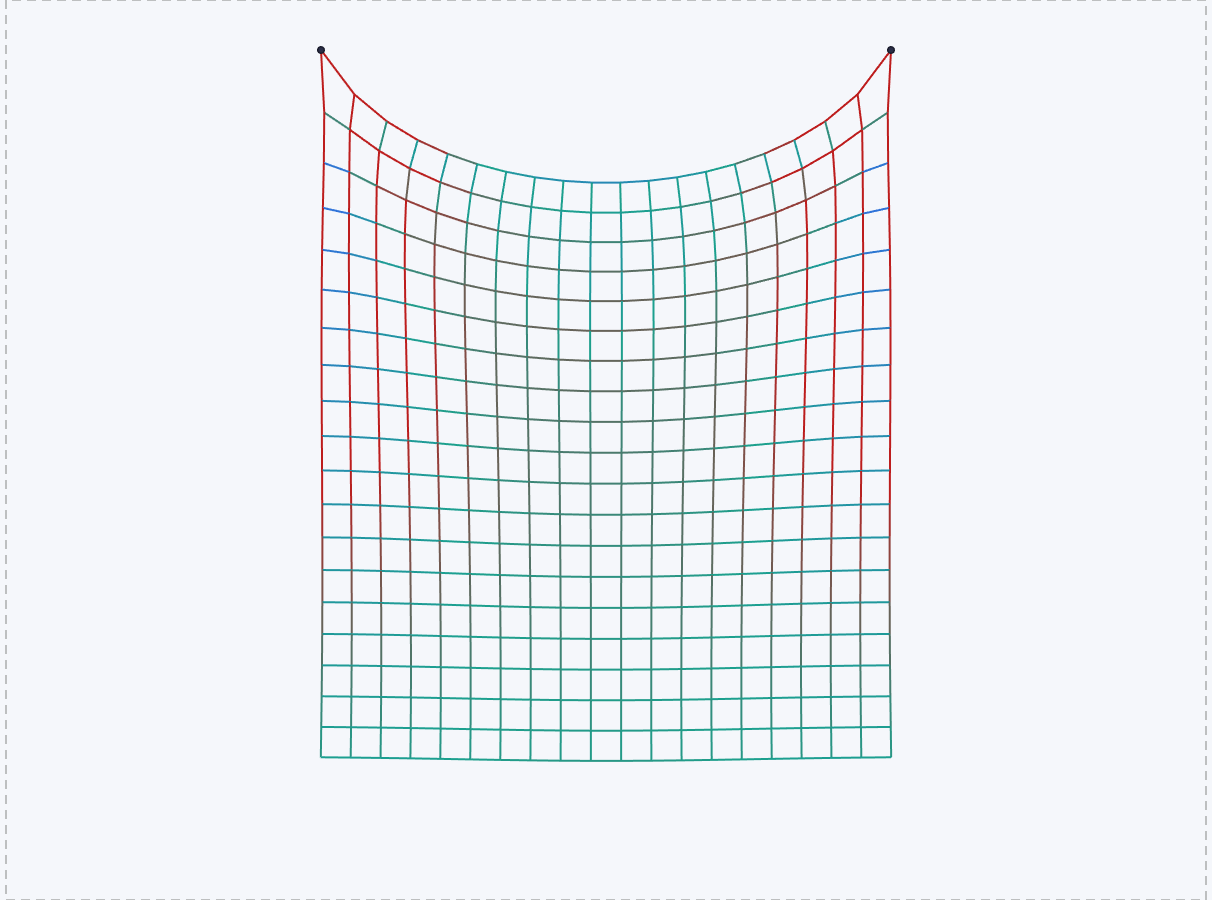
\includegraphics[width=0.66\linewidth]{../presentation/figures/scenes/scene_05.png}\\[1mm]
    {\small\color{textgrey}Un tissu de 400 particules et 1\,482 ressorts : les ressorts étirés rougissent, les comprimés bleuissent.}
  \end{center}

  \vfill
  {\large\bfseries\color{inpnavy} Léo DORVAL \textperiodcentered{} Nicolas MARCEL \textperiodcentered{} Audric SIGURET\par}
  \vspace{1mm}
  {\color{textgrey}Grenoble INP -- Phelma \textperiodcentered{} 3\textsuperscript{e} année SEI \textperiodcentered{} novembre 2026\par}
  \vspace{0.6cm}
\end{titlepage}

% ===================================================================== intro
\section{Introduction}

Ce projet consiste à écrire, en C++ et sans bibliothèque de physique, un moteur de simulation en deux
dimensions. Le monde y est peuplé de particules, c'est-à-dire de masses ponctuelles, que relient des
ressorts. Le moteur les anime en temps réel dans une fenêtre, et l'utilisateur peut les attraper à la
souris pour les lancer ou les épingler.

La physique en jeu reste simple. À chaque pas de temps, chaque particule additionne les forces qui
s'exercent sur elle. La loi de Newton lui donne alors son accélération, $\vec a = \sum \vec F / m$.
Il reste à avancer dans le temps : c'est le rôle de l'intégrateur, qui calcule la nouvelle vitesse et
la nouvelle position au bout d'un pas $dt = 1/120$\,s.

Quatre forces sont modélisées. La première est le poids, $m\vec g$. La deuxième est le frottement de
l'air, $-c\,\vec v$, opposé à la vitesse. La troisième est un vent qui varie dans le temps. La dernière est le ressort amorti, qui agit entre deux particules
A et B séparées du vecteur $\vec d$ :
\[
  \vec F_A = \Big[\,\underbrace{k\,(\lVert\vec d\rVert - L_0)}_{\text{élastique}}
    + \underbrace{\rho\,(\vec v_B - \vec v_A)\cdot\hat d}_{\text{frottement interne}}\,\Big]\,\hat d,
  \qquad \vec F_B = -\vec F_A .
\]
Le premier terme est la loi de Hooke : le ressort tire ou pousse selon qu'il est plus long ou plus
court que sa longueur au repos $L_0$. Le second freine les oscillations, en s'opposant à la vitesse à
laquelle les deux extrémités s'écartent.

Le moteur propose deux intégrateurs, et l'on peut passer de l'un à l'autre en pleine simulation. La
méthode d'Euler semi-implicite met d'abord à jour la vitesse, $\vec v \mathrel{+}= \vec a\,dt$, puis
la position avec cette nouvelle vitesse, $\vec x \mathrel{+}= \vec v\,dt$. La méthode de Verlet ne
garde pas la vitesse : elle déduit la position suivante des deux précédentes,
$\vec x_{n+1} = 2\vec x_n - \vec x_{n-1} + \vec a\,dt^2$.

Enfin, les particules vivent dans une boîte. Lorsqu'une particule franchit un bord, elle est ramenée à
l'intérieur et sa vitesse normale change de signe. Elle est en même temps multipliée par un
coefficient de rebond $b$, compris entre 0 pour un bloc inerte et 1 pour un rebond parfait.

Au-delà de la physique, l'enjeu du projet est l'architecture. Le moteur doit être extensible : une
force, un intégrateur ou un affichage de plus doit s'écrire comme une classe de plus, sans retoucher
le code existant. La physique doit aussi rester indépendante de l'affichage, assuré ici par la bibliothèque SFML.
Le code compile avec les options \code{-Wall -Wextra -Werror}, sans le moindre avertissement, et ne
doit laisser fuir aucune mémoire.

Ce rapport présente d'abord la conception du moteur et les raisons de nos choix. Il décrit ensuite
son implémentation et la manière dont nous l'avons testé. Il revient enfin sur l'organisation de
l'équipe, avant de conclure.

% ===================================================================== conception
\section{Conception}\label{sec:conception}

\subsection{Le diagramme de classes}

Toutes les classes du moteur descendent d'une même racine, \code{Entity}, qui donne à chaque objet un
nom et un identifiant unique. La figure~\ref{fig:hierarchie} montre la hiérarchie complète. Trois
interfaces la structurent : \code{Force}, pour tout ce qui exerce une force sur une particule ;
\code{Drawable}, pour tout ce qui se dessine ; \code{Integrator}, pour les méthodes d'actualisation
des positions. Les classes concrètes viennent se brancher sous ces interfaces.

\schemafig{hierarchie}{Hiérarchie des classes du moteur. L'héritage virtuel est en rouge, les classes abstraites en pointillé.}

Le tableau ci-dessous résume le rôle de chaque classe.

\begin{center}\small
\begin{tabularx}{\linewidth}{@{}>{\color{inpnavy}}l X@{}}
  \toprule
  Classe & Rôle \\
  \midrule
  Entity & racine commune, qui porte un identifiant unique et un nom \\
  Drawable & classe abstraite de tout ce qui se dessine, avec ses couleurs \\
  Force & classe abstraite de toute force, qui sait calculer son effet sur une particule \\
  Gravity, Drag, Wind & le poids, le frottement de l'air et le vent \\
  Spring & le ressort amorti, qui est à la fois une force et un objet dessiné \\
  Particle & une masse avec sa position, sa vitesse, son rayon et la liste de ses forces \\
  Integrator & interface des intégrateurs, implémentée par Euler et Verlet \\
  World & le monde, qui possède particules, ressorts et intégrateur \\
  Renderer & l'interface de dessin, seul point de contact avec l'affichage \\
  \bottomrule
\end{tabularx}
\end{center}

\subsection{Un ressort est une force qui se dessine}

Le ressort est la pièce centrale du moteur, et la plus délicate à modéliser. Il agit sur ses deux
particules, ce qui en fait une \code{Force}. Il apparaît aussi à l'écran, ce qui en fait un
\code{Drawable}. Il hérite donc des deux, et les deux héritent eux-mêmes d'\code{Entity} : c'est
l'héritage en diamant de la figure~\ref{fig:diamant}.

Sans précaution, un ressort contiendrait alors deux sous-objets \code{Entity}. Il aurait deux
identifiants, et l'appel \code{getId()} deviendrait ambigu. Nous avons donc rendu l'héritage
d'\code{Entity} virtuel : un ressort ne contient plus qu'une seule \code{Entity}, partagée par ses deux
parents. Le gain est aussi mémoire. Comme \code{Entity} contient une chaîne de caractères, un ressort
passe de 144 à 112 octets.

\schemafig{diamant}{L'héritage en diamant de \code{Spring}, et son effet sur la mémoire.}

\subsection{Des forces choisies à l'exécution}

Chaque particule garde la liste des forces qui agissent sur elle, sous forme de références vers la
classe abstraite \code{Force}. Pour calculer son accélération, elle parcourt cette liste et appelle
\code{compute} sur chacune. C'est la liaison dynamique qui choisit, à l'exécution, le bon calcul :
celui du poids, du frottement, du ressort ou du vent.

\begin{lstlisting}
void Particle::apply_force() {
  if (!moovable) return;                        // particule epinglee
  accel = Vec2(0, 0);
  for (std::reference_wrapper<Force> f : acting_forces)
    accel += f.get().compute(*this) / mass;     // appel virtuel
}
\end{lstlisting}

Ce choix rend le monde aveugle au type des forces. \code{World} ne contient aucun test pour savoir s'il
manipule un ressort ou du vent. Un ressort, à sa création, s'inscrit lui-même dans la liste de ses deux
extrémités. Ajouter une force revient donc à écrire une classe dérivée de \code{Force}, puis à
l'attacher aux particules voulues. C'est ainsi que nous avons pu ajouter après coup le vent, sans
modifier une ligne du moteur.

Les calculs eux-mêmes s'écrivent comme les formules, grâce à la surcharge des opérateurs de la classe
\code{Vec2}. Additions, produits par un scalaire et produit scalaire s'y lisent directement. Les
paramètres passent par référence constante, ce qui évite les copies sans permettre de modifications.

\subsection{Des intégrateurs interchangeables}

L'intégrateur suit la même logique. Le type voulu est une valeur d'un \code{enum class}, que la fonction
\code{makeIntegrator} transforme en objet. Le monde reçoit cet objet sous la forme d'un
\code{std::unique\_ptr} vers l'interface \code{Integrator}. Il n'en connaît que la méthode \code{step},
et ignore s'il s'agit d'Euler ou de Verlet (figure~\ref{fig:integration}).

\schemafig[0.82\linewidth]{integration}{Changement d'intégrateur : un type énuméré, une fonction qui crée l'objet, une interface commune.}

Changer d'intégrateur en pleine simulation pose cependant une difficulté. Verlet a besoin de la
position précédente, qu'Euler n'utilise pas. Nous avons donc demandé aux deux méthodes de tenir cette
position à jour. La bascule, déclenchée par la touche I, se fait ainsi sans que les particules ne
sautent.

\subsection{Un propriétaire unique et des adresses stables}

Le monde possède tous les objets de la simulation, et les liens entre eux sont nombreux. Un ressort
garde deux pointeurs vers ses particules. Une particule garde des références vers ses forces. Ces
adresses doivent donc rester valides pendant toute la simulation.

Notre première version rangeait les particules dans un \code{std::vector}. Or un vecteur qui grandit
peut réallouer toute sa mémoire et déplacer ses éléments. Les pointeurs des ressorts devenaient alors
pendants, et les ressorts n'avaient plus aucun effet. Nous avons remplacé ce conteneur par une
\code{std::deque}, qui ajoute ses éléments par blocs sans jamais déplacer les anciens
(figure~\ref{fig:world}). Les ressorts sont rangés de la même façon.

\schemafig[0.86\linewidth]{world}{Le monde possède tout : des conteneurs qui ne déplacent pas leurs éléments, et une copie interdite.}

La même réflexion a guidé la règle des trois. Copier un monde obligerait à reconstruire tous ces liens
vers les nouveaux objets. C'est compliqué, et jamais utile : une scène se reconstruit à partir de sa
fonction. Nous avons donc préféré interdire la copie, en la déclarant supprimée. L'intégrateur, tenu
par un \code{unique\_ptr}, est libéré automatiquement avec le monde.

\subsection{Une physique indépendante de l'affichage}

Le moteur ne contient aucun en-tête de SFML. Il dessine à travers l'interface abstraite
\code{Renderer}, qui ne propose que deux opérations : tracer un cercle et tracer un segment. Seul le
dossier de rendu l'implémente avec SFML (figure~\ref{fig:architecture}). La bibliothèque physique
peut donc être réutilisée telle quelle avec un autre affichage, une sortie d'images SVG par exemple.

La même idée vaut pour les scènes. Une scène n'est qu'une fonction qui remplit un monde vide de
particules et de ressorts. En ajouter une ne touche pas au moteur. Cette séparation nous a beaucoup
servi lorsque nous avons multiplié les scènes de démonstration.

% ===================================================================== implementation
\section{Implémentation}\label{sec:impl}

\subsection{Structure du code}

Le code est réparti en quatre dossiers, chacun compilé par CMake en une bibliothèque statique. Le
dossier \code{physics} contient le moteur. Le dossier \code{scenes} contient les scènes de
démonstration, qui n'utilisent que le moteur. Le dossier \code{render} contient l'implémentation SFML
de \code{Renderer}. Le dossier \code{app}, enfin, contient le programme principal ainsi que nos outils
de mesure et de capture. Chaque classe a son en-tête et son fichier source.

\schemafig[0.86\linewidth]{architecture}{Les dossiers du projet : la physique ne connaît que l'interface \code{Renderer}.}

SFML est téléchargée et compilée par CMake au premier lancement, puis liée statiquement. Aucune
installation manuelle n'est nécessaire, ce qui nous a évité bien des soucis entre nos machines.

\subsection{Le parcours d'un pas}

La figure~\ref{fig:parcours} suit une simulation de bout en bout. Au chargement, une scène crée ses
particules et ses ressorts dans le monde. Ensuite, chaque pas enchaîne trois étapes : le calcul des
forces, l'intégration, puis l'application des contraintes de bord. Une fois par image, le monde est
dessiné.

\schemafig{parcours}{Les sept étapes d'une simulation, et la boucle à pas fixe qui les rythme.}

L'affichage tourne à 60 images par seconde, et la physique à 120 pas par seconde. Pour les accorder,
la boucle principale accumule le temps réel écoulé. Tant que la simulation est en retard sur ce temps,
elle avance d'un pas, puis retranche ce pas du temps accumulé. On obtient deux pas par image en
moyenne. Surtout, la physique ne dépend plus de la vitesse de la machine. C'est indispensable pour
Verlet, qui suppose un pas de temps constant.

La création d'une particule illustre notre usage des constructeurs (figure~\ref{fig:particules}).
Une particule peut se créer de trois façons, mais un seul constructeur fait réellement le travail. Les
deux autres lui délèguent, ce qui évite de dupliquer le code. Le rayon est une constante : il ne peut
être fixé que dans la liste d'initialisation.

\schemafig[0.9\linewidth]{particules}{Constructeurs délégués et liste d'initialisation d'une particule. Le compteur d'identifiants est partagé par toute la classe.}

\subsection{Gestion des erreurs}

Le premier filet de sécurité est le compilateur. Toutes nos cibles sont compilées avec
\code{-Wall -Wextra -Werror}, si bien qu'un simple avertissement bloque la compilation. Le projet
compile sans aucun avertissement. Ces options ne s'appliquent qu'à notre code, et non aux en-têtes de
SFML. Le typage nous aide aussi : les méthodes de lecture sont constantes, chaque redéfinition porte le
mot-clé \code{override}, et les choix d'intégrateur passent par un type énuméré plutôt que par un
entier.

À l'exécution, les opérations qui peuvent échouer le signalent. La recherche d'une particule par son
identifiant lève une exception \code{std::out\_of\_range} si celle-ci n'existe pas. La recherche de la
particule la plus proche de la souris renvoie un pointeur nul quand il n'y en a aucune.

La mémoire, enfin, est gérée sans \code{new} ni \code{delete} dans le moteur. Les conteneurs de la
bibliothèque standard et les pointeurs intelligents s'en chargent. Pour le vérifier, nous avons passé
le test sans affichage sous Valgrind, avec la recherche complète des fuites. Les 26 simulations
allouent environ 100\,Mo en 52\,867 allocations, toutes libérées. Valgrind ne relève ni fuite ni
erreur.
\begin{lstlisting}[language={},emph={}]
==3== HEAP SUMMARY:
==3==     in use at exit: 0 bytes in 0 blocks
==3==   total heap usage: 52,867 allocs, 52,867 frees, 103,097,250 bytes allocated
==3== ERROR SUMMARY: 0 errors from 0 contexts (suppressed: 0 from 0)
\end{lstlisting}

\subsection{Tests et outils de mise au point}

Notre premier test simule chaque scène pendant dix secondes, avec les deux intégrateurs. Il vérifie
que toutes les positions restent finies et que les vitesses restent raisonnables. Il ne dépend pas de
SFML et s'exécute en quelques secondes, ce qui permet de le relancer après chaque modification.

Ce test ne dit rien, cependant, de la justesse de la physique. Pour mesurer la précision du modèle,
nous avons écrit un second programme, qui calcule à chaque pas l'énergie totale du système :
$E = \sum \tfrac12 mv^2 + \sum mgh + \sum \tfrac12 k(\ell - L_0)^2$. Nous l'appliquons à des scènes
sans frottement ni amortissement. Dans la réalité, l'énergie y serait parfaitement conservée. Tout
écart à sa valeur initiale vient donc du calcul pas à pas. La figure~\ref{fig:energie} montre que cet
écart oscille sans dériver. Sur le pendule, il ne dépasse pas 0,7\,\%, bien en dessous du seuil de
5\,\% que nous visions. Le double pendule, chaotique et doté de ressorts très raides, s'écarte
davantage, mais l'écart reste borné.

\begin{figure}[htbp]\centering
  \begin{tikzpicture}
    \begin{axis}[width=7.6cm,height=4.4cm,title={Pendule},xlabel={$t$ (s)},ylabel={écart (\%)},
        xmin=0,xmax=10,ymin=-1.2,ymax=1.2,axis lines=left,grid=major,grid style={asttrack},
        tick label style={font=\scriptsize},label style={font=\small},title style={font=\small\bfseries,color=inpnavy},
        legend style={font=\scriptsize,draw=none,fill=white,fill opacity=0.85,text opacity=1},legend pos=south west,
        every axis plot/.append style={line width=1pt,mark=none}]
      \addplot[timaorange] table[x=t,y expr={(\thisrow{euler}/58.86-1)*100},col sep=comma]{../presentation/figures/data/energie_pendule.csv};
      \addplot[astblue,dash pattern=on 3pt off 1.5pt] table[x=t,y expr={(\thisrow{verlet}/58.86-1)*100},col sep=comma]{../presentation/figures/data/energie_pendule.csv};
      \legend{Euler,Verlet}
    \end{axis}
  \end{tikzpicture}\hfill
  \begin{tikzpicture}
    \begin{axis}[width=7.6cm,height=4.4cm,title={Double pendule (chaotique)},xlabel={$t$ (s)},
        xmin=0,xmax=10,ymin=-4,ymax=4,axis lines=left,grid=major,grid style={asttrack},
        tick label style={font=\scriptsize},label style={font=\small},title style={font=\small\bfseries,color=inpnavy},
        every axis plot/.append style={line width=0.8pt,mark=none}]
      \addplot[timaorange] table[x=t,y expr={(\thisrow{euler}/100.847-1)*100},col sep=comma]{../presentation/figures/data/energie_double_pendule.csv};
      \addplot[astblue,dash pattern=on 3pt off 1.5pt] table[x=t,y expr={(\thisrow{verlet}/100.847-1)*100},col sep=comma]{../presentation/figures/data/energie_double_pendule.csv};
    \end{axis}
  \end{tikzpicture}
  \caption{Écart relatif de l'énergie totale à sa valeur initiale, sur dix secondes sans frottement.}\label{fig:energie}
\end{figure}

Ce test d'énergie nous a révélé une erreur dans les rebonds. Une balle parfaitement élastique aurait
dû garder son énergie, or celle-ci variait à chaque contact avec un bord. Deux défauts se cumulaient.
D'une part, la balle qui avait traversé le bord était simplement reposée dessus. La distance parcourue
au-delà du bord était perdue, et l'énergie potentielle avec elle. D'autre part, Verlet déduit la
vitesse de la position précédente. Inverser la vitesse sans corriger cette position revenait à annuler
le rebond au pas suivant.

La correction traite ces deux points (figure~\ref{fig:contraintes}). La balle est renvoyée à
l'intérieur d'une distance égale à $b$ fois son dépassement, comme si elle avait rebondi pendant le
pas. Sa vitesse normale est inversée et multipliée par $b$. Sa position précédente est enfin recalculée
à partir de la nouvelle vitesse, pour que Verlet reste cohérent.
\begin{lstlisting}
if (p.pos.y - p.radius < y_min) {
  p.pos.y = y_min + p.radius + p.bounciness * (y_min - (p.pos.y - p.radius));
  p.speed.y = -p.speed.y * p.bounciness;
  p.previous_pos = p.pos - p.speed * dt;      // historique de Verlet coherent
}
\end{lstlisting}

\schemafig[0.5\linewidth]{contraintes}{Rebond sur un bord : la particule est replacée à l'intérieur et sa vitesse normale inversée.}

D'autres outils nous ont aidés au quotidien. Le titre de la fenêtre affiche l'intégrateur courant et
le nombre d'objets simulés. La pause et l'avance pas à pas permettent d'observer une simulation image
par image. La couleur des ressorts, qui rougissent quand on les étire et bleuissent quand on les
comprime, rend visibles les tensions. Enfin, un programme de capture rejoue chaque scène sans
interaction et en enregistre l'image : c'est lui qui a produit les illustrations de ce rapport.

\subsection{Le résultat}

Le moteur anime treize scènes, du simple pendule au tissu de quatre cents particules. La
figure~\ref{fig:scenes} en montre trois. Le rideau est soumis à une force non prévue dans le cahier des
charges initial : un vent dont la
vitesse est donnée par une fonction du temps, écrite sous forme de lambda. La roue de vélo est
dessinée par-dessus sa position de départ, en gris, ce qui fait voir son écrasement au contact du sol.

\begin{figure}[htbp]\centering
  \begin{minipage}[b]{0.32\linewidth}\centering
    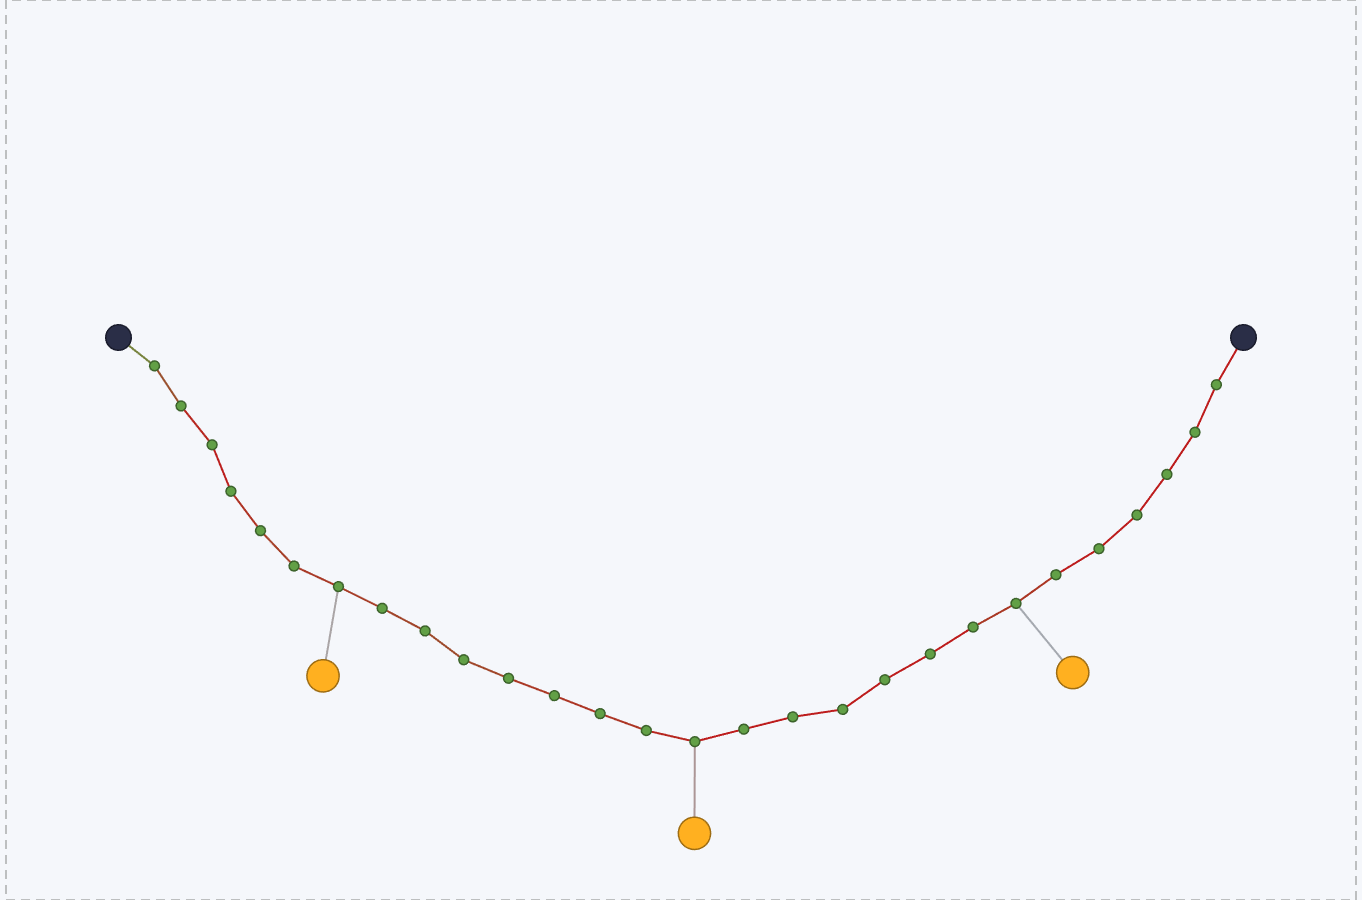
\includegraphics[width=\linewidth]{../presentation/figures/scenes/scene_04.png}\\[-0.5ex]{\small Pont de corde}\end{minipage}\hfill
  \begin{minipage}[b]{0.32\linewidth}\centering
    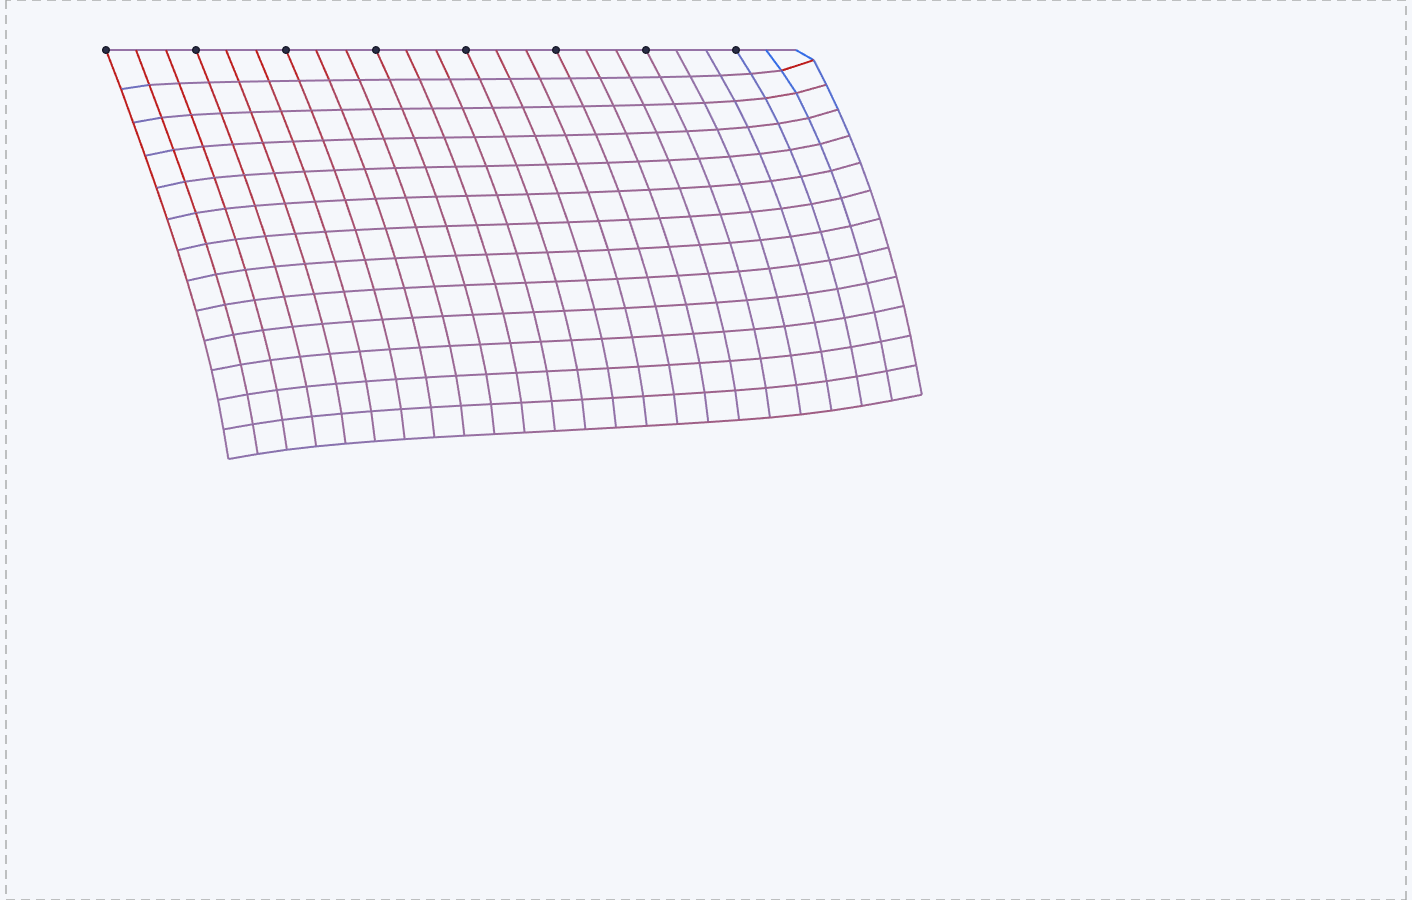
\includegraphics[width=\linewidth]{../presentation/figures/scenes/scene_07.png}\\[-0.5ex]{\small Rideau au vent}\end{minipage}\hfill
  \begin{minipage}[b]{0.32\linewidth}\centering
    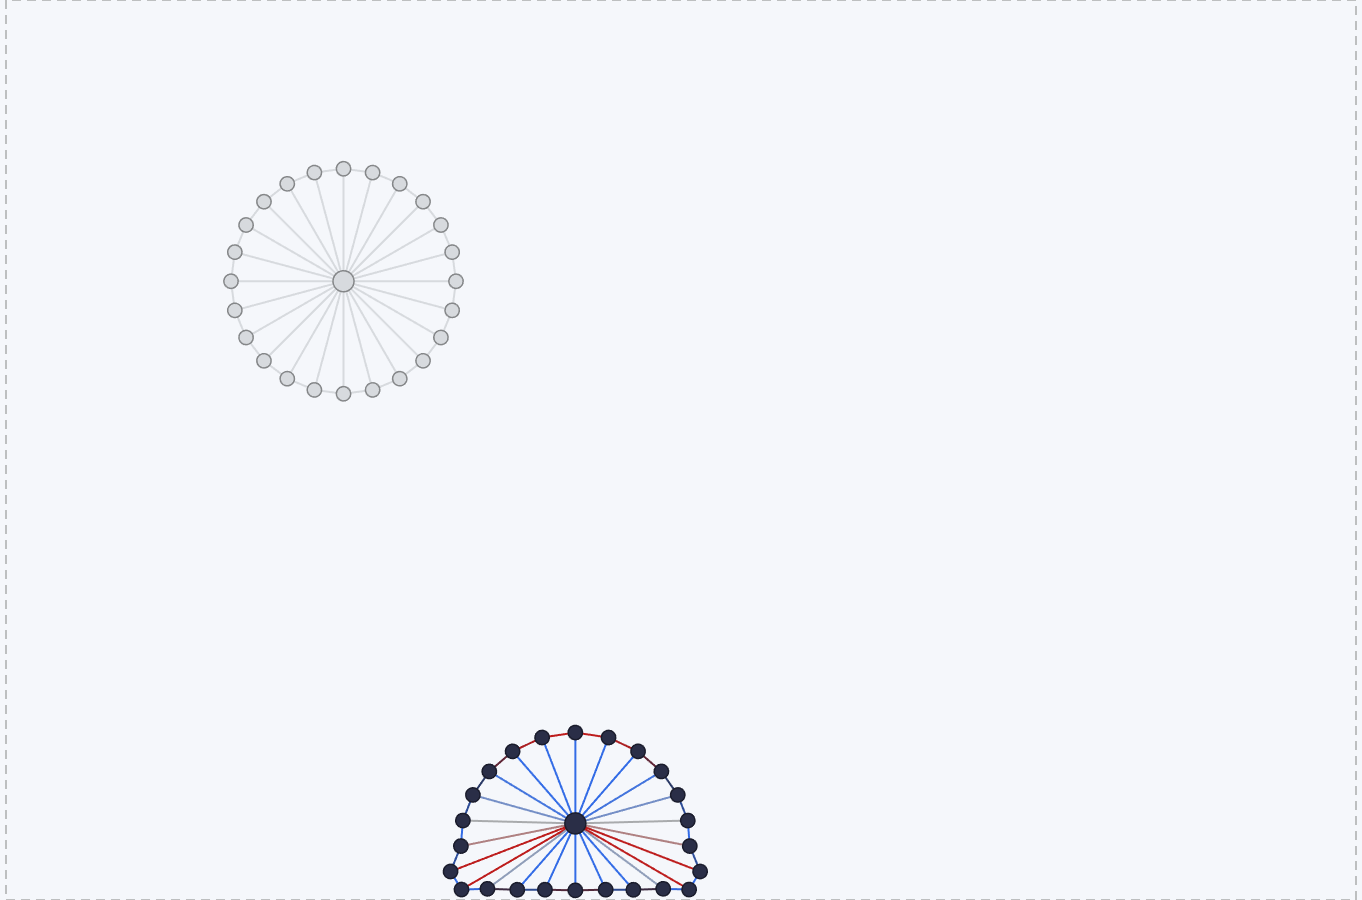
\includegraphics[width=\linewidth]{../presentation/figures/scenes/scene_06.png}\\[-0.5ex]{\small Roue de vélo}\end{minipage}
  \caption{Trois des treize scènes, capturées par le programme \code{capture}.}\label{fig:scenes}
\end{figure}

% ===================================================================== gestion
\section{Gestion du projet}\label{sec:gestion}

L'étape la plus importante du projet a été la toute première. Avant d'écrire la moindre ligne de
code, nous avons dessiné ensemble le diagramme de classes. Ces séances ont fixé les interfaces :
le calcul d'une force, le pas d'un intégrateur, le dessin d'un objet. Une fois ces contrats posés,
chacun pouvait avancer de son côté sans attendre les autres.

Nous avons ensuite découpé le diagramme en trois parts. Léo s'est chargé des forces et du
ressort. Nicolas a écrit les intégrateurs et le monde. Audric a pris en charge
\code{Entity}, les particules et le rendu. Chacun travaillait sur sa propre branche Git, avant de
fusionner son travail dans la branche principale du dépôt commun hébergé sur GitHub.

La mise en commun s'est faite sans difficulté majeure, précisément parce que les interfaces avaient
été décidées ensemble. Nous avons alors confié l'écriture des scènes de démonstration à l'assistant
Claude. L'objectif du projet était le moteur physique ; les scènes ne permettent que de montrer les
capacités du moteur physique.
Une dernière branche a enfin servi à préparer la soutenance et ce rapport.

Côté outils, CMake gère la compilation et le téléchargement de SFML. Les schémas ont été dessinés
avec draw.io, la présentation et ce rapport écrits en LaTeX. La figure~\ref{fig:gantt} retrace le
déroulement du projet, reconstitué à partir des dates des commits.

\begin{figure}[htbp]\centering
\begin{tikzpicture}[x=0.25cm,y=0.55cm,font=\footnotesize]
  % axe : jour 0 = 13 octobre, jour 37 = 19 novembre
  \foreach \d/\l in {0/13 oct.,8/21 oct.,18/31 oct.,27/9 nov.,37/19 nov.}{
    \draw[asttrack] (\d,0.4) -- (\d,-6.4);
    \node[text=textgrey,font=\scriptsize] at (\d,0.85) {\l};}
  \newcommand{\tache}[5]{% ligne, debut, fin, couleur, texte
    \fill[#4!60,rounded corners=1pt] (#2,-#1+0.32) rectangle (#3,-#1-0.32);
    \node[anchor=east,text=inpnavy] at (-0.4,-#1) {#5};}
  \tache{0}{0}{2}{inpnavy}{Lancement, sujet, CMake}
  \tache{1}{2}{8}{phelmared}{Diagramme de classes (ensemble)}
  \tache{2}{8}{18}{astblue}{World, intégrateurs, Entity, Particle, rendu}
  \tache{3}{26}{28}{datagreen}{Springs, rebond, séparation hpp/cpp}
  \tache{4}{28}{30}{dummyorange}{Mise en commun, scènes (Claude), correctifs}
  \tache{5}{29}{37}{sinkpurple}{Présentation et rapport}
  \tache{6}{29}{29.6}{timaorange}{Test d'énergie, bug du rebond corrigé}
\end{tikzpicture}
\caption{Déroulement du projet, reconstitué à partir des dates des commits Git.}\label{fig:gantt}
\end{figure}

% ===================================================================== conclusion
\section{Conclusion}

Nous sommes contents du résultat : à la fin, nous avons un moteur qui marche. Le modèle masses-ressorts
se comporte comme prévu, et il est physiquement juste, puisque l'énergie se conserve à moins de 1\,\%
près sur le pendule au bout de 5 oscillations. Les deux intégrateurs s'échangent en direct, et la hiérarchie de classes est restée
propre du début à la fin. Le moteur a aussi ses limites. Les particules ne se heurtent pas entre elles,
seulement contre les bords. Chaque ressort est calculé deux fois, une fois pour chacune de ses
extrémités.

Ce projet nous a fait pratiquer la programmation objet à une échelle réelle. Nous avons manipulé
l'héritage, y compris virtuel, le polymorphisme et les classes abstraites. Nous avons aussi découvert
des outils que nous ne connaissions pas. Les pointeurs uniques nous ont dispensés d'écrire le moindre
\code{delete}. La \code{std::deque}, avec ses adresses stables, a résolu notre premier vrai bug. Après
le C, le C++ nous a semblé bien plus confortable pour organiser un programme de cette taille.

Nous retenons surtout que la conception paie. Lorsque nous avons demandé à Claude d'ajouter des scènes
puis le vent, il n'a presque pas modifié notre code. Il s'est contenté d'utiliser les constructeurs et
les méthodes de nos classes, et le vent n'a demandé qu'une nouvelle classe dérivée de \code{Force}.
C'était exactement l'extensibilité que nous recherchions.

Quant à l'enseignement, un sujet ouvert comme celui-ci, où l'architecture compte plus que le nombre de
fonctionnalités, nous a obligés à penser les interfaces avant le code. C'est sans doute la leçon la
plus utile que nous en tirerons.

\end{document}
